\section{Tuesday, November 15th}
\subsection{Z Transform}
Today we will learn about the Z Transform which is for discrete time signals. The counterpart for continuous time signals is the Laplace transform.

\subsubsection{Time to wean off the unit circle}
We know from before that passing $x(n)=e^{i\omega n}$ into an LTI system gives out $y(n)=H(\omega)e^{i\omega n}$.

\begin{shaded}
Q: What if we pass in $x(n)=z^n=(re^{i\omega})^n$ into an LTI system. What do we get then for $y(n)$?
\end{shaded}

Using the definition -- the exact same way we did for the purely imaginary case -- we can say that:
\begin{align*}
    y(n) 
    &=
    \sum_{\ell} h(\ell)x(n-\ell)
    \\
    x(n) = z^n
    &\implies
    x(n-\ell) = z^{n-\ell}
    \\
    \implies
    y(n) 
    &=
    \sum_{\ell} h(\ell) z^{n-\ell}
    \\
    &=
    \sum_{\ell=-\infty}^\infty h(\ell) z^{-\ell} z^n
\end{align*}

Note that the first part of $y(n)=\underbrace{\left(\sum_{\ell=-\infty}^\infty h(\ell) z^{-\ell}\right)}_{\hat H(z)} z^n$ is a function of nothing other than $z$. It is not a function of $\ell$ as we sum over all $\ell$. 

Therefore, we call $\hat H(z)$ the \textit{transfer function of the system}. You will often see this written as: $\displaystyle\hat H(z)= \sum_{n=-\infty}^\infty h(n)z^{-n}$

\hrulefill

Now we can complete what we were saying before:

Passing in $x(n)=z^n$ into an LTI system gives out $y(n)=\hat H(z)z^n$.\\
In other words: sending in a complex exponential into an LTI system gives the same complex exponential scaled by the transfer function.

\textbf{We call $\hat H(z)$ the Z Transform of $h(n)$.} Most texts will just say $H(z)$ but we add the hat to avoid confusion when talking about the DTFT (which are denoted as $H$) along with Z Transforms (which are denoted here as $\hat H$).

\subsection{Region of Convergence}
Note: we only define $\displaystyle\hat H(z)\triangleq\sum_{n=-\infty}^\infty h(n)z^{-n}\ $ \textit{when the sum converges.}

Therefore we say that $z$ is in the Region of Convergence (ROC) if
\[
    \left|\sum_{n=-\infty}^\infty h(n)z^{-n}\right| < \infty
\]
Note that ROCs will always involve the absolute value of $z$.

\subsubsection{Aspects of Convergence}
\[
    z=re^{i\omega}
\]
\begin{shaded}
Q: Which aspect of $z$
\begin{itemize}
    \item $r$
    \item $\omega$
\end{itemize}
affects convergence?
\end{shaded}

The answer is $r$. $\omega$ does not affect convergence as it only exists within the term $e^{i\omega}$ which has magnitude 1. Or more rigorously:

\begin{align*}
    \left|\sum_\ell h(\ell)r^{-\ell}e^{-i\omega\ell}\right|&<\infty
    \\
    &\equiv
    \sum_\ell \left|h(\ell)r^{-\ell}\right|\left|e^{-i\omega\ell}\right|
    <\infty
    &&\text{[Magnitude of prod. = prod. of the magnitudes]}
    \\
    &\equiv
    \sum_\ell \left|h(\ell)r^{-\ell}\right|
    <\infty
    &&\text{$\left[|e^{-i\omega\ell}|=1\right]$}
\end{align*}

Note that the final expression $\sum_\ell \left|h(\ell)r^{-\ell}\right|<\infty$ has an $r$ in the LHS which appears in a potentially problematic manner:
if you have an impulse response that is growing, $r^\ell$ can contain the growth in the impulse response if chosen appropriately over an appropriate interval of $\ell$.

\subsubsection{Example of Convergence}
Let's give an example of choosing such an appropriate interval.

Say we have a causal system with $h(\ell)=2^\ell$. Then we can reformulate our condition to say that $\sum_{\ell=0}^\infty \left|(\frac 2r)^\ell\right|<\infty$, with the summation bounds following from causality. For this sum to converge, $\frac2r<1\implies r>2$. 
Taming choice example: If we take $r=3$, we will see that $\sum_{\ell=0}^\infty \left|(\frac 23)^\ell\right|<\infty$.

\subsubsection{Forms for Regions of Convergence}
Regions of Convergence can take on the following shapes, on the complex plane:
\begin{itemize}
    \item $R_0 < |z|$ (sometimes $R_0 < |z| <\infty$ to not include $z=\infty$): Regions of Convergence can be outside of some circle with radius $R_0$. Note that $R_0=0$ is possible in which case we include the entirety of the complex plane.
    \item $|z| < R_0$ (sometimes $0<|z|<R_0$ to not include $z=0$): Regions of Convergence can be inside of some circle.
    \item $R_0 < |z| < R_1$: the final possibility is if we have a donut.
\end{itemize}

\subsubsection{Duality of transforms of impulse responses}

Note that what we call the transfer function of the system is actually the Z transform of the impulse response.

Just like when we said that the frequency response of a system is the DTFT of the impulse response. 

\subsection{Why another Transform?}
Note there are signals that don't have a Fourier Transform (FT) but convolution is still well-defined.

We are familiar with the relationship (involving the DTFT) of sending in some $X(\omega)$ into a system $H(\omega)$ to get out $Y(\omega)=X(\omega)H(\omega)$. This however requires two things:
\begin{enumerate}
    \item the system, $H(\omega)$, has a frequency response
    \item the input has a DTFT
\end{enumerate}

However let us consider something new:\\
a system with impulse response $h(n)=2^n u(n)$ where your input is over a finite duration of 2 samples. Specifically $x(n)=\begin{cases}1 &\text{if n=0} \\ 2 &\text{if n=1} \\ 0 &\text{e/w} \end{cases}$.

We can see that convolution is well-defined here: $y(n)=\sum_{i=-\infty}^\infty h(i)x(n-i)=\begin{cases}1 &\text{n=0} \\ 2 &\text{n=1} \end{cases}$ \\
This is due to one of the signals being of finite length duration.

But you cannot talk about a FT since the system doesn't have a frequency response: \\
$H(\omega)=\sum_{n=0}^\infty 2^n e^{-i\omega n} =\sum_{n=0}^\infty (2 e^{-i\omega})^n$ but $|2 e^{-i\omega}|>1$ so the sum diverges for all $\ell_p$ norms $(\forall p)$. 
So while we do say that $h$ has no DTFT (so we can talk about the system in time -- via convolution -- but not in frequency), the system does turn out to have a Z Transform and so does the signal.

\subsection{Right-Sided Sequences}
\begin{shaded}
Definition:\\
We say a sequence $x$ is right-sided if $x(n)=0$ for all $n < N_0,\ \exists N_0 \in \mathbb Z$.
\end{shaded}
If we visualize a dot plot across $n$, then we will see that everything to the left of $N_0$ will be $0$ with lollipops only to the right.

In the case where $N_0=0$ then we are looking at a causal function.

\subsubsection{Convolution of 2 Right-Sided functions}
\begin{shaded}
Q: What if we have 2 right-sided signals $x, h$ and convolve them?
\end{shaded}

\[
    (x\ast h)(n) = \sum_{\ell=-\infty}^\infty x(\ell) h(n-\ell)
\]

We will have to keep one fixed (WLOG we shall keep $x(\ell)$ fixed here) and flip the other one (to get $h(-\ell)$) and then move it by some constant $n$ to get $h(n-\ell)$. \\
When we flip and move the \textit{right-sided} $h$, then everything non-zero moves from being to the right of some point $\ell=M_0$ to being only non-zero to the left of some different point $\ell=n-M_0$, with horizontal dotplot axes $\ell$. \\
Finally we multiply these 2 functions which leads to the following possible outcomes.\\
Either:
\begin{enumerate}
    \item $n-M_0$ (which is left-sided) is to the left $N_0$ (which is right-sided) in which case there is no overlap and the convolution \textbf{will yield 0.}
    \item Eventually as we increase $n$, the right-end of left-sided sequence will slide over the right-sided sequence and when we have overlap we will multiply pointwise.\\
    \textbf{This has finite overlap} due to the fact that they are extending in different directions and both sides have a stopping point $\Big(\ell=N_0$ for $x(\ell)$ and $\ell=n-M_0$ for $h(n-\ell)\Big)$.\\
    Finite overlap $\implies$ \textbf{finite output} once we've pointwise multiplied and summed.
\end{enumerate}
will occur.

\subsubsection{Example with Right-Sided functions}
\label{sec:ztransUnit}
Let's say you have some signal $x(n)=\left(\frac12\right)^n u(n)$. What is the Z Transform of this signal?\\
\textit{Hint: you will need to make use of $\ \displaystyle\sum_{n=0}^\infty \alpha^n =\frac{1}{1-\alpha},\quad |\alpha|<1$. \\Include constraints on $z$ for when the Z transform is defined: when its summation form converges.}
\begin{flalign*}
    \hat X(z) 
    &=
    \sum_{n=-\infty}^\infty x(n) z^{-n}
    &&\text{[Definition of Z Transform]}
    \\
    &=
    \sum_{n=-\infty}^\infty \left(\frac12\right)^n u(n) z^{-n}
    &&\text{[Plug in $x$]}
    \\
    &=
    \sum_{n=-\infty}^\infty \left(\frac1{2z}\right)^n u(n)
    &&\text{[Combine same exponential terms]}
    \\
    &=
    \sum_{n=0}^\infty \left(\frac1{2}z^{-1}\right)^n
    &&\text{[Use $z^{-1}$ notation, re-index per unit step]}
    \\
    &=
    \frac1{1-\frac12z^{-1}},\quad\left|\frac12z^{-1}\right|<1
    &&\text{[Use Hint; Introduce ROC constraints]}
    \\
    &=
    \frac1{1-\frac12z^{-1}},\quad|z|>\frac12
    &&\text{[Cleanup ROC constraints]}
\end{flalign*}

Therefore we can say that:
\begin{align*}
    x(n)=\left(\frac12\right)^n u(n)
    &\stackrel{\mathcal Z}\leftrightarrow 
    \hat X(z)=\frac1{1-\frac12z^{-1}},\quad R_x=\frac12<|z|
    \\
    x(n)
    &\stackrel{\mathcal Z}\leftrightarrow 
    \hat X(z)=\frac{z}{z-\frac12},\quad R_x=\frac12<|z|
    &&\text{[Multiply by $\frac zz$]}
\end{align*}

\subsection{Rational Z Transforms}
Note that this happens to be among the class of signals that have rational Z Transforms: This is rational in $z$ as it can be written as the ratio of 2 polynomials.

Roots of the numerator are called \textbf{zeros} of $\hat X$.\\
Roots of the denominator are called \textbf{poles} of $\hat X$.

In the above example, we have a zero at $z=0$ and a pole at $z=\frac12$.

We can give a pole-zero diagram by plotting the poles with X's and zeros with O's on the complex plane. ROCs are bounded by the poles as they can never include poles -- this is because poles are where things ``blow up'' as they are roots of the denominator. Zeros do not affect the ROC.

\subsection{DTFT Existence from Z Transforms}
In this case, we note that $ROC_x$ includes the unit circle which tells us that the DTFT exists:
Recall that we define
\begin{align*}
    \hat X(z)&=\sum_n x(n)z^{-n}
    \\
    &=\sum_n x(n)r^{-n} e^{-i\omega n}
    &&[z=re^{i\omega}]
\end{align*}
But if $r=1$ is inside the ROC then the above summation converges -- as then $z=e^{i\omega}$ is just somewhere \textbf{on} the unit circle. We will also notice that the $X(\omega)=\sum_n x(n) e^{-i\omega n}$ is the analysis equation for the DTFT as we plug in $r=1$.

More formally:
\[
    x(n)=\left(\frac12\right)^n u(n)
    \stackrel{\mathcal F}\leftrightarrow 
    \hat X(z)\left.\right|_{z=e^{i\omega}}=\frac1{1-\frac12e^{-i\omega}}
\]
which we will recall from our Fourier Transform days.

Note that we can only say $\hat X(z)\left.\right|_{z=e^{i\omega}}=X(\omega)$ if the ROC includes the unit circle.

\subsection{Z Transforms \texorpdfstring{$\to$}{->} DTFT Example}
\subsubsection{Z Transform with incorrect DTFT}
Let us find the Z Transform and then convert it into the DTFT for the signal $x(n)=u(n)$.

\begin{flalign*}
    \hat X(z) &= \sum_n u(n) z^{-n}
    &&\text{[Definition of Z Transform]}
    \\
    \hat X(z) &= \sum_{n=0}^\infty z^{-n}
    &&\text{[Re-index summation bounds per unit step]}
    \\
    \hat X(z) &= \sum_{n=0}^\infty (z^{-1})^n
    &&\text{[Introduce $z^{-1}$ term]}
    \\
    \hat X(z) &=\frac1{1-z^{-1}},\quad R_x = |z^{-1}|<1
    &&\text{[Geometric Series Convergence]}
    \\
    \hat X(z) &=\frac z{z-1},\quad R_x = 1<|z|
    &&\text{[Multiply by $\frac zz$ to find zeros/poles]}
\end{flalign*}

So we have a zero at $z=0$ and a pole at $z=1$, so our ROC extends outwards from the unit circle; however, it does not include the unit circle. \\
So \textbf{we cannot say} $X(\omega)=\frac1{1-e^{i\omega}}$ (in fact this is not the transform of the unit step function as $u(n)\not\in\ell_1, u(n)\not\in\ell_2, u(n)\in\ell_p \implies$ DTFT must have dirac deltas which we do not have).

\subsubsection{Correct DTFT}
The correct DTFT transform is
\[
    X(\omega)=\frac1{1-e^{-i\omega}}+\pi\delta(\omega),\quad \forall(|\omega|<\pi)
\]
with $2\pi$ periodicity. Note that $\frac12\stackrel{\mathcal F}\leftrightarrow \pi\delta(\omega)$ with normalization=1, oscillatory factor=-1 if you wish to verify with WolframAlpha.

We can wrap the $2\pi$-periodicity in one expression as:
\[
    X(\omega)=\frac1{1-e^{-i\omega}}+\pi\sum_{\ell=-\infty}^\infty\delta(\omega-2\pi\ell),\quad \forall\omega
\]


\subsection{Inverse Transforming}
\begin{important}
Note that there is an inverse Z Transform that we are going to treat as radioactive as it requires immense knowledge of Complex Analysis, Contour Integration, etc.
\end{important}
Therefore the inverse transforming that we do -- for both Z Transforms as well as Laplace Transforms -- will be limited to transform properties and known Z transform pairs.

\hrulefill

\subsection{Same but Different Z Transforms}
Given $q(n)=-\left(\frac12\right)^n u(-n-1)$, we know that $q(n)$ is non-zero for $-n-1\ge0$ or $n\le-1$. This is important to take care of as otherwise the unit step function will make $q=0$. Therefore it is non-zero for the first time at $n=-1$, with value $q(-1)=-2$ or $q(-1)=-\left(\frac12\right)^{-1}$. Then at the next time step $n=2$, we will maintain our negative sign but we shall grow our magnitude to have $q(-2)=-\left(\frac12\right)^{-2}$. And for all future negative timesteps, $q$ will continue to grow \textbf{exponentially}.

Since the $q$ is of exponential growth, we know that there will be no DTFT. This means that the $\text{ROC}_q$ must not include the unit circle. 
Finding the Z Transform:

\begin{flalign*}
    \hat Q(z)
    &=
    -\sum_{n=-\infty}^{-1} \left(\frac12\right)^n z^{-n}
    &&\text{[Re-index summation per modified unit step]}
    \\
    &=
    -\sum_{\ell=1}^{\infty} \left(\frac12\right)^{-\ell} z^{\ell}
    &&\text{[Change of variables: $\ell=-n$]}
    \\
    &=
    -\sum_{\ell=1}^{\infty} (2z)^{\ell}
    = -\left(\sum_{\ell=0}^{\infty} (2z)^{\ell} - 1\right)
    &&\text{[Combine, re-index]}
\end{flalign*}

This means we have 
\begin{align*}
    \hat Q(z) &= \frac{2z}{2z-1},\quad|z|<\frac12
    \\
    \hat Q(z) &= \frac{1}{1-\frac12 z^{-1}},\quad|z|<\frac12
\end{align*}
for our Z Transform, with the ROC being the exclusive circle extending inwards of radius $\frac12$.

Combining \hyperref[sec:ztransUnit]{with the earlier found Z transform\{u(n)\}}, we get that:
\begin{align*}
    \frac1{1-\frac12z^{-1}} \stackrel{\mathcal Z}\leftrightarrow
    \begin{cases}
        \left(\frac12\right)^n u(n) & \text{ if } |z| > \frac12
        \\
        -\left(\frac12\right)^n u(-n-1) & \text{ if } |z| < \frac12
    \end{cases}
\end{align*}
Note that the first case is stable -- as it contains the unit circle -- while the latter is not.

Looking at the pole-zero diagram, we see that the diagram is the same: \\
either way we have a zero at $z=0$ and a pole at $z=\frac12$. However the ROCs are different.

\subsection{ Generalizations from Causality to left/right-sided}
\begin{center}
    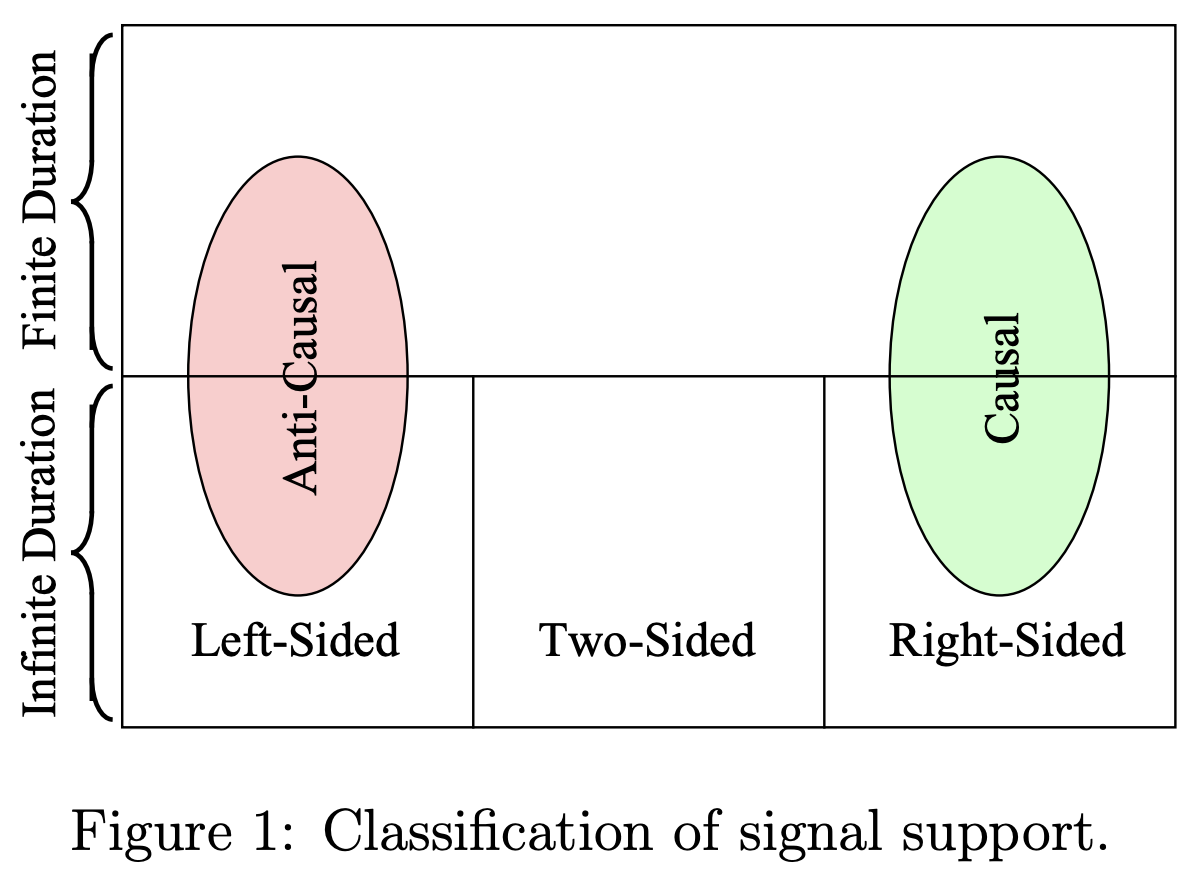
\includegraphics[scale=0.25]{lectures/wk12/img/signal_classification.png}
\end{center}

where an Infinite Right-sided Signal is Causal if the ROC includes $\infty$ and likewise for a Left-sided signal and the origin.

\subsubsection{Proof of Causal Extending}
For some causal signal $x(n)$ we know that any $R_1\in\text{ROC}_x$ will make the Z Transform converge by definition of the ROC (Region of Convergence). \\
Likewise since $R_1$ is in the ROC, we know it must be greater than the outermost.

So if
\[
    \hat X(R_1 e^{i\omega}) = \sum_{n=0}^\infty x(n) R_1^{-n} e^{-i\omega n}
\]
converges, then we know that \textit{any $R_2$} such that $R_2 > R_1$ will only make the summation converge faster. We can induct upon this idea and see there is no outer boundary to the radius.\\
$\therefore \hat X(R_2 e^{i\omega})$ certainly converges: if $R_1$ makes the sum converge then $R_2$ can too.

\subsubsection{Relationship between Time and Transform}
Note that the outermost pole is the pole that decays fastest and the ``dominant poles'' are the ones that decay slowest -- the ones that are away from the boundary. 

\subsubsection{Non-Causal Right-sided signals}
An example of such a signal lies within some signal $y(n)=\left(\frac12\right)^{n+1} u(n+1)=x(n+1)$. We can see that this signal $y$ starts at $n=-1$ and then for all future timesteps ($n=0,1,2,\ldots$), we see $y$ decay.

Finding the Z Transform:
\begin{align*}
    \hat Y(z) 
    &= \sum_{n=-1}^\infty y(n) z^{-n} 
    \\
    &= \underbrace{z}_{y(-1)(z^{-1})^{-1}} + \underbrace{\frac12}_{y(0)(z^{-1})^{0}}
    + \ast z^{-1} + \square z^{-1} + \cdots
\end{align*}
where the $\ast$ and $\square$ coefficient terms are irrelevant garbage.

As $z\to\infty$, the first term blows up. Even though we have a right-sided signal, the very first term (aka one lollipop on the dotplot which causes problems) leads to us not being causal.

Therefore the ROC$_y = \frac12<|z|<\infty$ where we exclude infinity to denote that we are not causal.

\subsubsection{Anti-Causal and Left-sided signals}
If you have an anti-causal signal you grow inwards including the origin.

But left-sided signals that are not anti-causal go all the way to the origin but do not include it.

You will see more nuances of this in the homework: problem set 10.

\subsection{ RoC Causality and Left/Right-sidedness Summary}
\begin{itemize}
    \item Causal RoC: $R_0<|z|$
    \item Right-sided but not causal RoC: $R_0<|z|<\infty$
    \item Anti-causal RoC: $|z|<R_0$
    \item Left-sided but not anti-causal RoC: $0<|z|<R_0$
\end{itemize}
\begin{shaded}
Q: Is the exclusion of 0 important as it means the constant signals cannot be included?
\end{shaded}
A: No, constant signals are $|z|=1$.

\subsubsection{Anti-Causality vs Non-Causality}
Anti-Causal ($h(n)=0,\forall n>0$) is always one-sided 
whereas non-causal can also be two-sided (donut shaped RoCs).

\subsection{ Mixing Z Transforms}
Anytime you mix Z Transforms, you have to make sure the RoCs have a non-trivial overlap.\\
Otherwise, one or the other is not convergent.

\subsubsection{Mixing Z Transforms Example}
\begin{align*}
    x(n)
    &=\left(\frac12\right)^n u(n) - 2^nu(-n-1)
    \\
    x(n)
    &\stackrel{\mathcal Z}\leftrightarrow
    \frac1{1-\frac12z^{-1}} + \frac1{1-2z^{-1}}
    \\
    \text{ROC}&=\quad\frac12<|z|\ \cap\ |z|<2
    \\
    \hat X(z)
    &=\frac z{z-\frac12} + \frac z{z-2}
    \\
    &=\frac{2z(z-\frac54)}{(z-\frac12)(z-2)}
    &&\text{[Common denominator $\to$ factor]}
    \\
    \text{ROC}&=\quad\frac12<|z|<2
\end{align*}

This is a non-causal (or 2-sided) decaying exponential signal.

\begin{shaded}
Sanity Check: Since each of the 2 parts of $x(n)$ is absolutely summable (as they are decaying exponentials), we know that the ROC must include the unit circle which it does!
\end{shaded}

\subsection{ Convolution in Time}
Let us feed in $x(n)=z^n$ to system $h(n)$ (which internally is a composition of $f(n)$ sent into a $g(n)$) to get out $y(n) =\hat H(z)z^n$.

This means that $z^n$ is also an eigenfunction of an LTI system, just like $e^{i\omega}$ was but now you are not restricted to being on the unit circle.

Breaking it down, step-by-step, we see that:\\
$f(n)$ gives out $\hat F(z)z^n$\\
which is sent to $g(n)$ which gives out $y(n)=\hat F(z)\hat G(z) z^n$.

Pattern matching to before, we see that $\hat H(z)=\hat F(z)\hat G(z)$.

\begin{shaded}
Big idea: Convolution in Time $\mapsto$ Multiplication in the Transform domain (just like with FT).
\end{shaded}

\subsection{ Generalization of Convolution in Time}
If we pass $x(n)$ into a system $h(n)$ to get $y(n)=(x\ast h)(n)$.

Then $\hat Y(z) = \hat X(z)\hat H(z)\implies \hat H(z)=\frac{\hat Y(z)}{\hat X(z)}$.

\subsection{ Time-Shift Property}
For a signal $x(n)$ with a Z Transform, let us define $y(n)\triangleq x(n-N)$.

This shall have Z Transform: $\hat Y(z)=\hat X(z)z^{-N}$ which you know from you incredible EE120 Prof!
\begin{align*}
    \hat Y(z)
    &= \sum_{n} x(n-N) z^{-n}
    &&\text{[Definition of Z Transform]}
    \\
    &= \sum_{\ell} x(\ell) z^{-(\ell+N)}
    &&\text{[Change of Variables: $\ell=n-N\implies n=\ell+N$]}
    \\
    &= \sum_{\ell} x(\ell) z^{-\ell} z^{-N }
\end{align*}
This is why we saw delay blocks written as $z^{-1}.\hfill\square$
